
\section{OSI-Modell}
\subsection{Dienst}
{Klassifizierung von Diensten:}
\begin{center}

    \begin{tabular}{ | l | l |}
        \hline
        Verbindungsorientiert & verbindungslos    \\ \hline
        \makecell{Verbindungs-Aufbau nötig        \\ Ziel muss bereit sein} &
        \makecell{ Jederzeit Nachrichten schicken \\ Ziel muss nicht «bereit» sein} \\   \hline
    \end{tabular}

\end{center}
\begin{center}
    \begin{tabular}{ | l | l |}
        \hline
        Zuverlässig & Unzuverlässig          \\ \hline
        \makecell{Kein Datenverlust          \\ Sicherung durch \\Fehler-Erkennung \\ -/ Korrektur} &
        \makecell{ Möglicher Datenverlust    \\ Keine Sicherung} \\   \hline
        \makecell{  Text-Nachrichten, Backup \\ Dateidienste} & \makecell{Streaming \\ Voip}     \\   \hline
    \end{tabular}
\end{center}
\vfill\null
\columnbreak
\subsection{Schicht}
{Eine Schicht hat die Aufgabe der darüberliegenden Schicht bestimmte
    Dienste zur Verfügung zu stellen. Die Schichten benötigen kein Wissen über die Realisierung
    der darunterliegenden Schicht.

        {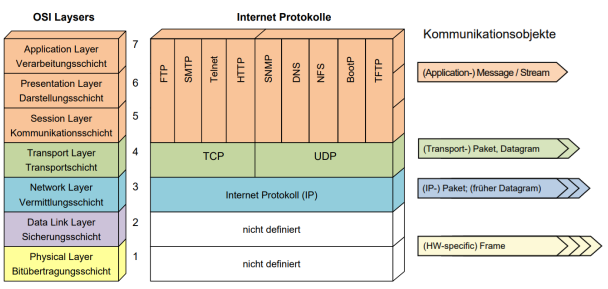
\includegraphics[scale=.4]{img/osi-1.png}}

        {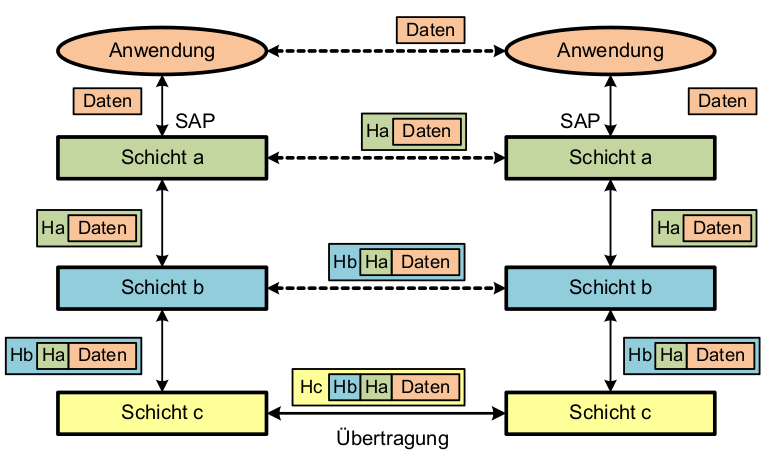
\includegraphics[scale=.3]{img/osi-2.png}}}
\subsection{Protokoll}
{Ein Protokoll ist eine Sammlung von Nachrichten, Nachrichtenformaten und Regeln zu deren Austausch.
    In der Technik ist ein Kommunikationsprotokoll eine Vereinbarung, die festlegt wie eine Datenübertragung zwischen Kommunikationspartnern abläuft.}
